\chapter{身份}

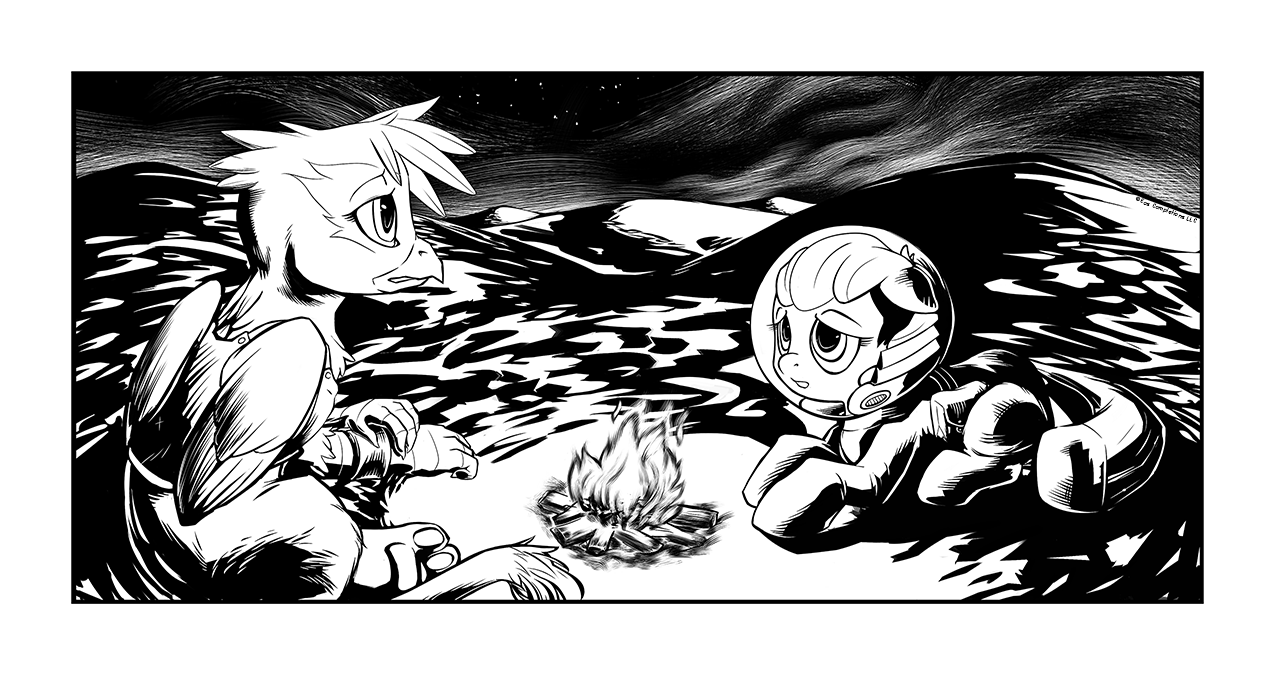
\includegraphics[width=0.9\linewidth]{image10.png}

\begin{intro}
在沙漠之中你要铭记自己的名字,因为没有一位马不会给你带来伤害。
\end{intro}

\daytimeplace{9}{2:00 AM}{太阳城市区,52号国道中段}{Sun City Downtown, Big 52 SC Branch}

「肏你妈,老娘头疼得都睡不着……」赫瑞塔揉着她的脑袋,帕比丢石头的时候不但瞄得挺准,而且力气也不小,现在狮鹫正在为帕比长时间锻炼的丢石头技巧埋单。在一整天的繁重体力劳动,比如拆房子,搬砖头啥的之后,狮鹫已经累得足以倒头就睡了——如果她的脑袋没有隐隐作痛的话。

「下次我见到那个黄色小恶魔的话,我要打她屁股打到她坐不下去。」说起来,那小东西在太阳城做什么?这个城市就是个陷阱,那个嗡嗡的洗脑声……

赫瑞塔一瞬间睁大了眼睛,「等等……那肏狗的嗡嗡声……没有了?老娘终于可以正常思考和喷脏字儿了!」半鹰站起来张开了翅膀正准备离开,但是下一瞬间看着她的几个室友呆住了,这个房间里有五只狮鹫,其中两个是一路把她追到这里的鹰爪,另外三个也纹着鹰爪的纹身,但是没有穿制服和铠甲。

「终于轮到老娘的复仇回合了……」赫瑞的喙上浮现出一个冷笑,然后拔出自己的匕首。她慢慢朝一只熟睡的狮鹫逼去,那只狮鹫既没有铠甲也没有武器,和她一样因为一整天的繁重体力活而睡得死死的。年轻的狮鹫像是草丛中的蛇一样无声无息地接近她的猎物,慢慢举起她爪子中闪着寒光的凶器……然后这个复仇者看到了那个狮鹫怀中的蛋。

「日你老母的……」看到紧紧抱着两个蛋熟睡的狮鹫,赫瑞塔眼眸之中的复仇怒火熄灭了。狮鹫迟疑着,她并不忍心杀死一个熟睡之中的母亲……但是另外四个就是……

另外四个又怎么样呢?他们也是这里的牺牲品,其中之一还可能是这些蛋的父亲,而且他们现在手无寸铁,还在熟睡之中,就算追着她的那两个狮鹫醒来,她也早跑到几公里之外了,在这里流血又有什么意义呢?

「肏你妈,老娘才不是背后捅谁刀子的懦夫……」赫瑞塔转身走向门口,不过她注意到屋子角落的一个粉色东西。是叫什么来着?丝袜?马尾啥的……反正是那家伙的玩偶。淦,差点忘记带上这东西,「哦,我了个擦!帕比!」她差点忘记带上那个死小孩儿!

\horizonline

\daytimeplace{9}{2:30 AM}{太阳城中心,52号国道中段}{Sun City Downtown, Big 52 SC Branch}

坐在漆黑的控制室里面,帕比依然不明白发生了什么,她完全不知道在声音先生回来之前,那个雌驹的声音是什么,不过她很确定那也是个漂漂马。不过只要想想那个可怕母马的声音在她脑中回响的感觉,就让帕比觉得不寒而栗。

不过很幸运,帕比现在状态很好,不管那个雌驹的声音干了什么事,最重要的是,先给她起个好听的名字,不过声音小姐已经用过了……

「啊……她就是她,小姐就是小姐,不过她就有点……呃……吓马?所以……鬼音?听起来好奇怪……」帕比皱了皱眉头,这个可真是个难题。「头音?不对……梦魇之音?太长啦……我知道了!怕音,因为她怕怕!耶!」

头盔的HUD上闪过一条提示,告诉帕比,任务:『梦魇现身』已经完成,没错,帕比太厉害了!她无所不能的!起个名字这种事情当然难不倒她。不过这么老长一段看不懂的字还是有点挑战性……而且数数超过自己的蹄子数量也有点儿……而且打开花生酱瓶子也……基本是不可能完成的任务……不过没关系,到现在为止她基本遇上的都是简单模式,所以出发吧!帕比!

好了,给自己打气结束,计划第一部分也完成,现在是计划的第二部分,找到赫瑞,然后像落叶赛跑中的小马一样快跑离开这里。

「好咯好咯!声音先生,赫瑞在哪?」

「{\mt 赫瑞塔·火红已经被设定为主要目标。}」

罗盘上的箭头消失,然后出现在帕比左边,箭头旁边表示距离的数字则快速的减少着。

「耶!冒险时……」

乒!

咣当!

乒!

一扇窗户被打碎的同时,年轻的飞行员拍打着翅膀,双爪紧握两把.45手枪,在飞溅的玻璃碎片之中冲进控制室。「坚持住帕比!」狮鹫在半空中两枪打碎了在EMP冲击之后刚刚恢复的灯泡,然后在一片漆黑中一个前滚翻躲在了桌子后面,这一连串的动作一气呵成。

突然出现的精彩表演看得帕比脸上露出惊讶的表情,哇塞,酷毙了!赫瑞绝对是最厉害的小马!简直就像电影中出来的英雄一样!小小雌驹在地板上踏着前蹄为她的朋友喝彩:「呀呼!冲啊赫瑞!你好厉害!太漂亮了!」接着一连串的子弹差点打中帕比的头盔。

「你丫干啥呢帕比,给老娘趴地上!我来解决那些肏蛋货!滚出来啊吃脑子的混蛋!」

「啥?」小雌驹一脸不解地歪着头。

发现这个屋子完全没有还击的对手,赫瑞尴尬地笑着,停止了扮演突击队员的角色,把枪放回枪套,用爪子按了按头顶的羽毛,想让自己看起来比较酷。

「嘿,帕比,没缺蹄子少尾吧?」

幼驹低头数了数自己的蹄子和尾巴,然后点了点头,「我都带在身上呢!丝尾没事吧!」

「你的玩偶?哦,你想要吗?」赫瑞拿出粉色的毛绒玩具晃着,而帕比摇了摇头。

「才不要咧,她和你在一起很好,我让她看着你,她还警告我说你有危险,所以我来这里救你但是你做着鬼脸骂了我然后又不理我所以我等到入夜之后执行我的超绝密潜入计划去告诉镇长这镇子烂透了但是我来到这里之后发现镇长不是镇长而是个傻蛋声音还说我的坏话但是我比他聪明所以他说很抱歉然后跑掉了,所以——我比蓝声音聪明!\footnote{这里类似于S01E12里苹果丽丽对云宝黛西说话的语速,节奏也一样}」

赫瑞塔举起一只爪子:「等等等等等!你他喵的嘴动那么快老娘一个字都没听清都就听你吧啦吧啦!都什么乱七八糟的,而且也没那闲工夫听你逼逼,赶紧麻溜地过来,这地方现在挤满了英克雷的杂毛和鹰爪的狮鹫,还有不知道天杀的什么势力的马——全都坐在一大堆新鲜食物和干净的饮水上。」

帕比疑惑地玩着头,「呃……那么,然后呢?」

狮鹫无奈地用爪揉着脑门,「好吧,长话短说,几小时之后这里就要变成个大战场了,在此之前我们要赶紧溜号,懂?」

「战场?就是小马们互相伤害的地方?」帕比有点疑惑地问。

「对,你丫可算是对了一回,每堆小马都想要把好东西全都占为己有,所以赶紧把口袋里没用的死重的东西都丢了,在被炸上天之前要赶紧飞离这个火药桶。」

帕比皱着眉头,「但是为什么要争斗,小马应该是漂漂而且好好的,打架是不对的,我们要爱与宽容……」小幼驹说着她的简单生存理念。

赫瑞塔正想反驳说就是这爱与宽容把小马国变成现在这么个大粪坑,但是她也明白这可不是和帕比斗嘴的时候,「对,没错,但是在你丫被『爱与宽容』之前还是快点闪……呃……你不是还得找你妈妈么?」

帕比点了点头,「对啊!我要去那个什么天麻肥鸡场什么的地方,但是漂漂姐姐和我说那里叫……啊……我不记得名字了,不过罗盘上有个箭头我绝对不会错过的!」

赫瑞塔叹了口气,「我猜,这地方在天杀的南边吧。」狮鹫伸出爪子指着。

帕比惊讶地看着她的朋友,「哇哦,你怎么知道的?你是魔法师么?」

「没错,老娘可是小马国最伟大的魔术师,天下无双的赫瑞……现在赶紧的!把你的破烂都倒出来。」狮鹫顿了顿,然后看着她朋友问,「话说,你什么时候给鬃毛染了个蓝条?」

一缕蓝色的鬃毛在帕比额前闪闪发光的金发之中格外显眼,就在她右眼上,这道鬃毛看起来就像是一道夜空的剪影一般,让赫瑞塔想起来自己见过的那什么魔法部的招贴画,那个叫暮光傻傻还是什么的家伙。

\horizonline

\daytimeplace{9}{3:00 AM}{太阳城中心,52号国道中段}{Sun City Downtown, Big 52 SC Branch}

帕比大着胆子睁开一只眼睛看了看下面,地面在夜空中飞快地向后滑去,高大的大厦看起来就像是火柴盒一样,布满灰尘的公路就在她鼻子下面快速地移动——不过距离她鼻子实在太过遥远到让她不舒服。

「我我我我我们还没到吗啊啊啊!!」小雌驹用力抱紧赫瑞塔的脖子,狮鹫觉得自己快要被掐死了。

「呃!松开你丫的蹄子!想让老娘陪你一起坠机么?」

一开始带着帕比飞还很顺利,这个小家伙丢掉身上的垃圾之后,重量还不如一个背包沉。可是当帕比发现她恐高之后,麻烦就开始了……{}

「你就闭上眼睛,当做自己是在骑小马啥的!」

帕比把自己眼睛闭得就像是避难厩的大门一样,但是完全没有用,一想到那些房子,树木啥的飞快地移动得就像是一团模糊的水彩一样,帕比就……「拜托,拜托!拜托我会做个乖孩子!放人家下啊啊啊啊啊!」

「我勒个擦,你丫至少对你朋友的飞行技术有点信心好不好!」赫瑞塔用力拍打了一下翅膀,然后从两座高楼之间的缝隙穿了过去,远远离开太阳城,清凉的夜风带着海水的味道,今晚绝对是个飞行的好夜晚——如果没有背上这个吵闹的包袱的话。

「你丫给老娘放松点儿!可以唱点歌什么的嘛!」

唱点歌,帕比觉得这个意见听起来不错!只要唱个歌一切都会好起来!小雌驹清了清嗓子然后开始唱。

「
\begin{song}
    蛋头蛋头坐墙上
    
    蛋头蛋头摔地
\end{song}

……啊啊啊啊拜托拜托拜托拜托拜托放!人!家!下!来啊啊啊啊啊!」

作为一个狮鹫,一个掠食者,在她远古的血液中,赫瑞是很高兴抓着一只在她双爪之中挣扎的小马猎物,但是一个在她脑袋上跳舞的幼驹就是另一回事了。「你丫给我安静!不会让你掉下去的,所以别惹老娘发火!……也别扯毛!你这死丫头知道背上的羽毛长回来要花多长时间吗!?」被帕比惹火的年轻飞行员把小雌驹从背上甩下来,然后用前爪紧紧抓住。「这回至少不会掉下去了!飞出废墟就给你放下。」

「咿……呀……!」

「小鬼别尿裤子,还要飞几公里呢,我们最好在那个大号火药桶炸上天之前离开这地方。」半鹰兽说着加快速度,用尽全力拍打着翅膀,她们俩就像是『嚎哭女妖』一样划过夜空,惊醒了沿途的所有小马,赫瑞塔祈祷着没有小马探出头寻找声音的来源。

\horizonline

\daytimeplace{9}{3:30 AM}{蛇蝎沙漠,52号国道中段}{Serpent Desert, Big 52 SC Branch}

「其实人家一点也不害怕,你懂的……只是……只是那啥……呃……看着那么多房顶,吹着风,然后有点……嗯……稍微有点兴奋……尤其是不知道你往哪儿去的时候。」四个蹄子都接触到了结结实实的地面之后,帕比正在为了挽回自己的面子而拼命辩解。不过从赫瑞塔笑得满地打滚的状态看来,这努力完全没有效果。

「活宝,你真是个活宝!」狮鹫在狂笑声之中吸了一口气,擦了擦眼泪,然后又爆出另一阵大笑。「你怎么尖叫的?咿……!再来啊,再叫一次我听听!」

黄色的小雌驹噘着嘴坐在地上叹了口气说:「哼,是谁在这城里迷路啊……小鸡你真是……」

乒……

帕比低头看着她黄色外套上胸口位置的一个大洞,喊了起来:「我说,那么多坏机器打我还不够啊?!」

赫瑞塔毫不在意地在爪子上转着自己的手枪,依然止不住刚才的大笑,「抱怨个屁啊,你丫给蝎尾狮扯成碎片都没事,老娘再给你开俩洞又能怎样?」

乒!乒!

又有两发子弹穿过帕比,一发打在蹄子上,一发打在胸口,「别闹了好吗!每次衣服有洞这破衣服都会念叨个没完!」在狮鹫打出的洞上露出了一丝粉色的气体。

「好吧,不过丫的别叫老娘小鸡好吗?」打了个哈欠,赫瑞塔收起了手枪,「顺便提醒你,普通小马甚至尸鬼被子弹开个洞都会死……所以别和其他小马玩这个游戏,好么?」

帕比点点头,然后又有点疑惑地歪着头,「但是我也是个普通小马,我是小马!」

「喂喂,我说你不是……喂,怎么忽然这个表情了?你是想让我唱个摇篮曲么?」赫瑞塔一脸调侃的表情问。

小雌驹开心地点了点头,「当然!我超超超超超爱摇篮曲!我们可以一起唱《静悄悄甜蜜蜜》吗?」

狮鹫一脸不爽地以爪覆面,该怎么才能告诉这个小雌驹她只是在调侃而已,「你真是麻烦,帕比……」

\begin{song}
「静悄悄,甜蜜蜜,该是安睡的时间!


\begin{englishlyric}
    ``Hush now, quiet now, it's time to lay your sleepy head!
\end{englishlyric}

\medskip

静悄悄,甜蜜蜜,还是入眠的时间!」 \footnote{这是正剧S01E17中的歌词}


\begin{englishlyric}
    Hush now, quiet now, it's time to go to beeed!''
\end{englishlyric}
\end{song}

赫瑞叹口气继续往南走,「为什么,老爹啊,老娘怎么就欠了这个傻蛋两次!」然后她笑着回过头说:「你坐上你的红滑板车吧,我在你头上飞,如果你想明天之前到那边的话,我们还有很多路要赶呢。」

\horizonline

\daytimeplace{9}{10:30 PM}{蛇蝎沙漠,52号国道中段}{Serpent Desert, Big 52 SC Branch}

帕比和赫瑞塔围在小小的营火边,她们的影子落在远处的沙丘上,赫瑞塔正在吃着一个锡罐里面的食物,从她的表情可以看出那东西显然不适合狮鹫的饮食习惯。沙漠上空的厚厚云层让这里在夜间也很温暖,但是那个半鹰依然穿着她的铠甲。

「这么说,那个蓝声音什么的说你是机器?」

赫瑞的表情看起来有些微妙,似乎是想在幼驹说完整个故事之前努力保持一副扑克脸。

「对,而且他听起来非常确定……我差点也信了,但是另一个怕音告诉我那是不可能的,因为……呃……我不明白她说的到底是什么,不过听她说的话应该没有问题。」帕比睿智地点了点头,就好像她什么都懂一样。

狮鹫耸了耸肩,「那么说,一个电脑说你是某种疯狂机器马,然后又有个幻觉说你不是……我觉得你肯定是被那EMP弹震晕了,然后EMP残存在你防护服电路里面的静电让你做了一个噩梦。」赫瑞塔打了一个哈欠,继续说:「不过我可不觉得你是机器……机器挨枪子儿会爆炸……而且,机器聪明多了。」

幼驹皱着眉头,「那你觉得我是什么?」

半狮子蹲坐在地上抓着自己的后腿,「你?反正对于我来说你不是啥好事……不过我喜欢你,所以你可以跟老娘混,叫『大姐姐赫瑞』。」

帕比走到她伙伴面前,直视着赫瑞塔双眼,幼驹的双眸在夜空中就是两个亮亮的粉色光源。「哦……但是……我是小马,对吧?我是说,就算我不吃东西不喝水而且还不上厕所,但是我还是小马?对吧?我是小马吧……」

\emph{她看起来忧心忡忡的样子,这个机器马什么的事情看起来真的吓到她了,不过……真他喵的肏蛋,为啥是老娘收拾烂摊子?}赫瑞现在完全精疲力竭,最不想见到的就是个打破砂锅问到底的幼驹,她现在只想要睡觉。哈欠连天的狮鹫拍着幼驹的头盔,「你是什么都不重要,帕比,你是个善良的小马,在废土上善良的小马很难见,只要你还认为自己是小马,你就是小马,所以……睡觉吧,拜托。」

幼驹开心地笑了。隔着头盔蹭了蹭赫瑞塔。

「谢谢你赫瑞,你是我最好的小鸡朋友!」

坐在她熟睡的伙伴身边,帕比叹着气,她一点都不困……

……

……

「喂!你说我因为机器很聪明所以我不是机器是什么意思!」帕比生气地戳着狮鹫的屁股,但是赫瑞只是轻笑一声然后转过身去。

「活宝。」

小马不停地戳着她的朋友想要听到回答,但是狮鹫开始大声打起了鼾,留下无奈的帕比独自坐在快熄灭的营火边。

\daytimeplace{10}{1:00 AM}{蛇蝎沙漠,52号国道中段}{Serpent Desert, Big 52 SC Branch}

寂静的黑夜之中帕比毫无倦意,幼驹一点都不觉得累,但是赫瑞现在不想被打扰,所以幼驹做了她自己觉得最合理的事情,在沙漠的夜晚上放哨,因为帕比最聪明了!

不过这里和帕比的期待根本对不上。那么多牛仔电影里面,沙漠应该都是骷髅,箭头,风滚草还有各种乱七八糟的东西,但是在『真正』的沙漠之中走了几天之后,帕比觉得那些水牛估计都休假去了,而且这里一只蝎子或者蛇都没看到,怎么可以叫蛇蝎沙漠呢?她目所能及之处只能看到几辆马车的残骸,还有一个看起来像是大号贪吃灵之类的东西在不远处闲逛,不过她靠近的时候,那些贪吃灵为了躲避她都飞走了。

「{\mt 警告,发现敌对生物。分析中,变异贪吃灵。威胁等级:致命。}」

「哎,为什么这里所有的毛茸茸生物都这么害羞?我只想交个朋友!」活了两百年的老怪物对着自然母亲和污染父亲联姻突变的小怪物说。

「嗨帕比,好久不见,你可真是跑了好远啊,不是吗?」一个金属的声音打断了小幼驹的小小探险,小可爱开心地笑着转向她的朋友。

「提问者先生!你去哪里啦?」

「是守望者,我守望着废土,守望……」

「好啦好啦,提问者先生,」帕比点着头微笑着,「我也可以守望什么吗?」

机器精灵发出金属质的窃笑,「帕比,帕比从未改变\footnote{这里改编自 \emph{FoE: PH} 的名句「战争,战争从未改变」}……你最近还好吗?我听说你在隧道镇有个小小冒险,而现在你已经跑到太阳城南边了。」

「没错!见到了好多漂漂马!有个叫赫瑞的小鸡,还有阿索和甜花,乐乐姐,还有好多好多朋友!」

「哇哦,你有这么多朋友,真幸运,不是吗?说起来,你去太阳城了?」声音想要保持一个稳定的音调,但是却透出一股好奇。

帕比皱了皱眉头,「对啊,就像一个用丝带包着的超级棒的礼物盒,但是里面却塞着燕麦……大家都一脸不开心,而且不和我聊天不和我玩,他们的镇长是个笨声音只会说可怕的话。」

「什么可怕的话?你想和我说说看吗?」

守望者的声音现在听起来很担心。

帕比看着远处说:「他说我不是小马是机器,然后我用那个可以让机器睡觉的大茶壶让他睡了,但是我也不能动……大家都说我不是机器,但是为什么……」

「呦呦,帕比,别烧坏你的小脑子,我可以很确定地说你不是机器,那个声音估计读取了一些感应器数据,但是它只是个看不懂小马心灵的机器,你也是个漂漂马,懂吗?现在对我笑笑,别再去想咯。」

帕比点点头,轻轻地笑了。

「非常好,满城的僵尸马……你找到什么发出兹兹或者类似轰鸣声的东西么?」

「没啥,但是赫瑞和我说那个吱吱声已经消失了,所以那些漂漂马会醒来然后做不漂漂的事情。」

「哦,终于那自律智能不见了,我终于可以看看里面……我想,又是你做的吧?」

帕比皱了皱眉头,「不,我只是听说赫瑞有危险所以过来……但是她没有,而且像个傻鸡一样飞来飞去不理我,和城里其他小马一样,所以我去找镇长声音和她吵了一架,然后他说我是傻瓜于是我拿出蓝色大茶壶……」

「呃……抱歉,蓝色大茶壶是啥?」

幼驹叹了口气,用蹄子扶着头盔,「为啥我每次都要从头解释?就是一个茶壶,圆圆的,亮亮的,还有个蓝色尖头!我在一个沼泽的破烂车车里面找到的!」

「好吧,所以你在一台超级计算机面前引爆了一个EMP震荡弹,的确,搞定那自律智能的又是你……话说你鬃毛怎么了?」

帕比歪着头想要看自己的鬃毛,「你说那个蓝条?我不知道,我一醒来就……」

「嘿帕比,那是谁?我就来!」赫瑞的声音打断了小马。

「抱歉小家伙,我要走了,你下次可以和我讲这个故事。」不等她回答,机器精灵发出一阵静电啪啪声,就继续开始播放音乐了。

狮鹫双爪各持一把枪落在沙丘上,不过她发现这里没什么威胁之后,双枪少女收起武器训斥着帕比,「坏孩子!别和机器精灵玩儿,回营地来。」

帕比和漂浮的机器挥了挥蹄子,然后回到了她朋友身边,「我没玩儿,我只是和他说我的超级大冒险!」

「对,对,对,我们回去睡觉吧,明天还要走很远呢。」狮鹫揉了揉帕比的头盔然后回到营地。

一个半小时之后,吓坏的肉食灵终于从隐蔽之处出来继续建造它的巢穴。

\horizonline

{\rt 雌驹们,公马们,早上好!这里是孤狼的52电台!你敢说废土还有比我这里更好的电台么?谁?DJ PON-3?拜托,我听说他只是个雌驹,不骗你们,而且在晴朗之夜她还会变成三头钻石犬!我不骗你们,只要在晴朗夜晚去十马塔就能看到!不过L.P.我很确定废土不会有什么晴朗之夜,或者晴朗之日。不过这不是我的错小马们,你们继续听52电台,别管什么DJ了!

好吧,回到新闻时间!昨天早上太阳城从19年的长眠之中醒来,我不知道具体发生了什么,不过看起来在晚上有谁袭击了城市的中央控制塔,摧毁了不知道谁放在那里的洗脑电台。没错小马们,你们没听错,以前太阳城是不归之地是因为那里完全被洗脑电波控制了!简直是疯狂!

你们猜那些住民意识到洗脑电波结束之后他们干了什么?你没猜错,他们开始继续相互残杀企图夺取城镇,如果你想穿过蛇蝎沙漠,跟着东边的绿色路径绕道,远离太阳城,重复一遍,尽可能远离太阳城!

好吧,大家可能还要问,谁是撤换城市管理员的家伙?还用得着我说那个名字吗?没错,伙计们,我们的小小英雄把你们从永无止境的噩梦中拯救出来,而你们还把你们的生命继续浪费在互相杀戮这种无聊的事情上!你们还有廉耻没有?我……算了,不提也罢,我们还是听会儿音乐吧。

现在即将播放的是:永不可及……}

 DJ的声音被音乐代替。

\begin{music}
看着你的孩子争斗。

\begin{englishlyric}
    Look at you young colts fighting.
\end{englishlyric}

\medskip

看着你的女儿哭泣。

\begin{englishlyric}
    Look at your fillies crying.
\end{englishlyric}

\medskip

看着你的儿女死去,

\begin{englishlyric}
    Look at your young colts dying,
\end{englishlyric}

\medskip

正如往昔一样。

\begin{englishlyric}
    The way they've always done before.
\end{englishlyric}
\end{music}

\horizonline

\daytimeplace{10}{10:30 AM}{铁锈庄园,52号国道中段}{Rust Manor, Big 52 SC Branch}

铁锈庄园看起来和它的名字一模一样,不知道是谁用巨大天空马车残骸建造了一个超级大号的路障,在不远处可以看到屹立在沙漠之中的兵营和空管塔,整个建筑都被强化钢板覆盖着,但是现在所有的金属都被锈迹侵蚀,看起来这里严重缺乏维护。不过,此地只是个小小的交易站,几辆篷车就在小镇外面,北边的大门附近有很多卫兵在地面和城墙的塔楼上巡逻。

远在几公里之外,赫瑞塔就叫帕比停了下来,毕竟在战争期间这里也是个军事要塞,不过这里的建筑除了空管塔楼基本都被炸毁了,所以这里的一片空地非常适合塔楼上的狙击手控制整个区域。

「等等,红箭!」狮鹫降落在小雌驹面前,让她在一团烟尘之中刹车。

「哇啊!看好降落地点啊!我差点撞上你!」

「我知道啦,好了,你丫这个鱼缸脑袋仔细听好,我现在要走了,不过这里很安全,你不会有麻烦的。」

帕比睁大了水汪汪的眼睛哀求着。「为什么?我不想你走啊!」

「我知道,我超酷的,没有老娘你丫啥都不是,不过那些在太阳城追我的家伙估计已经在这里等我了,我不想把你卷入麻烦。」

「哼!如果有坏小鸡追你,我们可以和他们解释你是个好孩子,然后和他们道歉他们就不会惹你了吧。好么?」

赫瑞塔叹了口气拍了拍帕比的头盔,「故事比你想象得复杂,毕竟我爆了他们好几个伙计的脑袋,所以他们现在在追我,所以……没戏,我可不觉得我们道个歉就能解决问题,而且我也不想道歉,他们杀了我父亲。」

「哦……」帕比低下头,想着其它解决办法,「你不能欺负那些欺负你的孩子,我是说哦,他们不是坏机器,他们是漂漂猫,你不能欺负小猫猫!」

赫瑞塔嗤之以鼻,「没错,漂漂猫……所以我不想进城,如果我不进去,我也没必要去把他们揍到不能再欺负我为止。」狮鹫耸了耸肩,「不管怎么说,照顾好自己,帕比,我们很快会再见了。」不等帕比回答,赫瑞塔就在一阵沙尘之中飞上了天空。

幼驹追着她的朋友跑了几百米,大叫着她,「唉,这不公平,她都没和我吻别……」幼驹看着天空尖叫着,「丝尾,照顾好她,她现在归你负责啦!」

\horizonline

\daytimeplace{10}{11:00 AM}{铁锈庄园,52号国道中段}{Rust Manor, Big 52 SC Branch}

狙击手在瞄准镜之中看着那个黄色的点,但是独角兽雌驹不太确定她看到的是什么,于是她把蹄子按在了对讲机上,「这里是坚守,一一八六处有情况,看起来是一个穿黄衣服的小马,或许是无线电里面说的小幽灵,看起来很像……我们这里欢迎幽灵么?」

对讲机传来了回复:「继续注意目标,如果你看到敌对举动再报告,否则让她继续靠近。」

「了解!」雌驹回到她的守备位置。

同时,帕比来到了前面,引起了大门外所有卫兵的注意,很多小马都相互窃窃私语着,举起了武器。不过小雌驹完全没有留意他们的举动,她只知道妈妈或许在那个镇子里面!

「嗨!我是快乐帕比!你们看到我妈妈了么?声音先生说她在这里!」

所有的小马都看着小雌驹,然后其中之一叹了口气,「没错,这个就是孤狼说的小幽灵。」卫兵放下他们的武器继续各忙各的去了。不过没有小马回答她的问题。

「呃……我想,你们是说没有吧。」幼驹一脸狐疑,发觉自己再次被忽略,于是她喃喃自语着:「求马不如求己,好吧声音先生,我们该去哪儿?」

「{\mt 分析中,读取本地地图,蓝羽机场,无法匹配,读取备份资料,寻找可能地点,地点找到:中央控制塔。中央控制塔被设定为下一个目标点」罗盘的箭头开始转向。}」

「哦,在城里!好!」帕比转头走向大门,但是马上被一个穿着雇佣兵铠甲的老公马拦住了,他眼中的神情帕比觉得很熟悉,她想起来曾经见过这一幕。

\rcpr{「喂喂,妈妈,为什么那个小马只有三条腿?」}

\rcpr{「她是战斗英雄,帕比,别打扰他,他已经很累了。」}

\rcpr{「说得没错,把我的腿献给破烂女神的破烂敌人,老子不知道那些破烂煤值得那么多小马去死么?」}

\rcpr{「哦……漂漂马说了奇怪的话!」}

\rcpr{「帕比,别听他胡说,那些都是坏话!你也是,和一个小孩子讲粗口害不害臊?」}

\rcpr{「滚边去婊子……」}

\rcpr{「我们走吧,帕比,跟我来,」}

\rcpr{「但是妈……我想要……」}

\rcpr{「死粉老鼠,找你妈哭去!没啥好看的!」}

帕比眨了眨眼,沉浸在回忆中,当她回过神来的时候,那个愤怒眼神的老马依然站在那里,小雌驹战战兢兢地走过去,「嗨……你见过我妈妈么?」

佣兵啐了一口,「你聋了?」

幼驹坐下来,有些疑惑地看着骂她的马,「呃……很抱歉我没听到你说什么……为什么你那么生气?我做错什么了吗?」

雄马轻蔑的笑着,「我问你丫是不是觉得自己是个英雄啥的?」

帕比微笑起来,这个问题简单。「我是太空战士安德洛队长!只要有我的太空服和超快飞车,我可以跑遍整个世界交很多很多好朋友!想和我玩么!我还有一个火箭!」小雌驹举起蹄子说:「火箭!」一个火箭玩具飞到了小雌驹面前。

老马抬起一根眉毛。「你把我当傻子吗?你知道老子是谁么?别在这里装逼,找肏是不是?」

帕比咯咯笑着,奇怪的话总是逗她笑,「哦……漂漂老马说奇怪的话了,我能一起玩吗?我会造词!比如说,滑板爪子!或者香蕉电话!」

那群小马开始大笑起来,小雌驹不知道他们在笑什么,不过她也一起跟着笑起来……不过这样下去迟早某马会血溅沙漠。

坚守又一次把蹄子按在对讲机上,「坚守报告,北门外面的佣兵队有麻烦了,那黄色小马看起来要和佣兵打起来了。」

「我们派卫兵去解决,在我们没有被攻击之前不要轻举妄动!」

「收到!」

这时老马抓着帕比的蹄子把她拎了起来,凶恶地看着她,「你刚嘲笑老子?就是因为电台里面的傻货吹嘘几次,你丫是不是觉得自己天下无敌了?」

「喂,放下我,我要找我妈妈!我又没惹你,大坏蛋,放我下来!」幼驹挣扎着,但是却没法挣脱,「我妈妈如果在的话她一定会教训你的,放开,放开我!」

或许是孩子的哭声让紧张的气氛消失了,那群小马有些尴尬地别开了脸,那个老佣兵也不知道自己到底在干啥,这个小丫头不是什么看起来超级厉害的英雄,穿着闪闪发光的骑士铠甲在城市间执行什么只有露娜才知道的神圣任务,她只是个……「肏蛋,孤狼绝对是脑子进了水才会觉得这个智障儿童是个英雄。」

这时候帕比开始哭了,哇哇地大哭,没有小马想去看这么没面子的事情。

佣兵叹了口气把幼驹放地上,「滚边去,老子不打小孩。」他轻哼一声,帕比转头哭着跑掉了。

在内心深处,他觉得自己也像是个坏蛋,而且为此而羞耻不已,不过那也只是一瞬间罢了。

~\vfill

\begin{note}
升级(Lv 9)

新技能解锁:哭泣公主——你可以用哭泣来解决几乎所有问题,你可以解锁特别对话选项来避免战斗,不过你会因此而损失声望。
\end{note}



